 %===============================================================================
% LaTeX sjabloon voor de bachelorproef toegepaste informatica aan HOGENT
% Meer info op https://github.com/HoGentTIN/latex-hogent-report
%===============================================================================

\documentclass[dutch,dit,thesis]{hogentreport}

% TODO:
% - If necessary, replace the option `dit`' with your own department!
%   Valid entries are dbo, dbt, dgz, dit, dlo, dog, dsa, soa
% - If you write your thesis in English (remark: only possible after getting
%   explicit approval!), remove the option "dutch," or replace with "english".

\usepackage[inkscapeformat=png]{svg}
\usepackage{float}

\usepackage{lipsum} % For blind text, can be removed after adding actual content

%% Pictures to include in the text can be put in the graphics/ folder
\graphicspath{{../graphics/}}

%% For source code highlighting, requires pygments to be installed
%% Compile with the -shell-escape flag!
%% \usepackage[chapter]{minted}
%% If you compile with the make_thesis.{bat,sh} script, use the following
%% import instead:
\usepackage[chapter]{minted}
\usemintedstyle{solarized-light}

%% Formatting for minted environments.
\setminted{%
    autogobble,
    frame=lines,
    breaklines,
    linenos,
    tabsize=4
}

%% Ensure the list of listings is in the table of contents
\renewcommand\listoflistingscaption{%
    \IfLanguageName{dutch}{Lijst van codefragmenten}{List of listings}
}
\renewcommand\listingscaption{%
    \IfLanguageName{dutch}{Codefragment}{Listing}
}
\renewcommand*\listoflistings{%
    \cleardoublepage\phantomsection\addcontentsline{toc}{chapter}{\listoflistingscaption}%
    \listof{listing}{\listoflistingscaption}%
}

% Other packages not already included can be imported here

%%---------- Document metadata -------------------------------------------------
% TODO: Replace this with your own information
\author{Mattias Verscheure}
\supervisor{Dhr. J. Courtens}
\cosupervisor{Dhr. J. De Graeve}
\title{Dreigingsanalyse en dreigingswaarschuwing a.d.h.v. netwerkflow data.}
\academicyear{2024--2025}
\examperiod{1}
\degreesought{\IfLanguageName{dutch}{Professionele bachelor in de toegepaste informatica}{Bachelor of applied computer science}}
\partialthesis{false} %% To display 'in partial fulfilment'
%\institution{Internshipcompany BVBA.}

%% Add global exceptions to the hyphenation here
%\hyphenation{back-slash}

%% The bibliography (style and settings are  found in hogentthesis.cls)
\addbibresource{bachproef.bib}            %% Bibliography file
\addbibresource{../voorstel/voorstel.bib} %% Bibliography research proposal
\defbibheading{bibempty}{}

%% Prevent empty pages for right-handed chapter starts in twoside mode
\renewcommand{\cleardoublepage}{\clearpage}

\renewcommand{\arraystretch}{1.2}

%% Content starts here.
\begin{document}

%---------- Front matter -------------------------------------------------------

\frontmatter

\hypersetup{pageanchor=false} %% Disable page numbering references
%% Render a Dutch outer title page if the main language is English
\IfLanguageName{english}{%
    %% If necessary, information can be changed here
    \degreesought{Professionele Bachelor toegepaste informatica}%
    \begin{otherlanguage}{dutch}%
       \maketitle%
    \end{otherlanguage}%
}{}

%% Generates title page content
\maketitle
\hypersetup{pageanchor=true}

%%=============================================================================
%% Voorwoord
%%=============================================================================

\chapter*{\IfLanguageName{dutch}{Woord vooraf}{Preface}}%
\label{ch:voorwoord}

%% TODO:
%% Het voorwoord is het enige deel van de bachelorproef waar je vanuit je
%% eigen standpunt (``ik-vorm'') mag schrijven. Je kan hier bv. motiveren
%% waarom jij het onderwerp wil bespreken.
%% Vergeet ook niet te bedanken wie je geholpen/gesteund/... heeft

%%=============================================================================
%% Samenvatting
%%=============================================================================

% TODO: De "abstract" of samenvatting is een kernachtige (~ 1 blz. voor een
% thesis) synthese van het document.
%
% Een goede abstract biedt een kernachtig antwoord op volgende vragen:
%
% 1. Waarover gaat de bachelorproef?
% 2. Waarom heb je er over geschreven?
% 3. Hoe heb je het onderzoek uitgevoerd?
% 4. Wat waren de resultaten? Wat blijkt uit je onderzoek?
% 5. Wat betekenen je resultaten? Wat is de relevantie voor het werkveld?
%
% Daarom bestaat een abstract uit volgende componenten:
%
% - inleiding + kaderen thema
% - probleemstelling
% - (centrale) onderzoeksvraag
% - onderzoeksdoelstelling
% - methodologie
% - resultaten (beperk tot de belangrijkste, relevant voor de onderzoeksvraag)
% - conclusies, aanbevelingen, beperkingen
%
% LET OP! Een samenvatting is GEEN voorwoord!

%%---------- Nederlandse samenvatting -----------------------------------------
%
% TODO: Als je je bachelorproef in het Engels schrijft, moet je eerst een
% Nederlandse samenvatting invoegen. Haal daarvoor onderstaande code uit
% commentaar.
% Wie zijn bachelorproef in het Nederlands schrijft, kan dit negeren, de inhoud
% wordt niet in het document ingevoegd.

\IfLanguageName{english}{%
\selectlanguage{dutch}
\chapter*{Samenvatting}

\selectlanguage{english}
}{}

%%---------- Samenvatting -----------------------------------------------------
% De samenvatting in de hoofdtaal van het document

\chapter*{\IfLanguageName{dutch}{Samenvatting}{Abstract}}


%---------- Inhoud, lijst figuren, ... -----------------------------------------

\tableofcontents

% In a list of figures, the complete caption will be included. To prevent this,
% ALWAYS add a short description in the caption!
%
%  \caption[short description]{elaborate description}
%
% If you do, only the short description will be used in the list of figures

\listoffigures

% If you included tables and/or source code listings, uncomment the appropriate
% lines.
\listoftables

\listoflistings

% Als je een lijst van afkortingen of termen wil toevoegen, dan hoort die
% hier thuis. Gebruik bijvoorbeeld de ``glossaries'' package.
% https://www.overleaf.com/learn/latex/Glossaries

%---------- Kern ---------------------------------------------------------------

\mainmatter{}

% De eerste hoofdstukken van een bachelorproef zijn meestal een inleiding op
% het onderwerp, literatuurstudie en verantwoording methodologie.
% Aarzel niet om een meer beschrijvende titel aan deze hoofdstukken te geven of
% om bijvoorbeeld de inleiding en/of stand van zaken over meerdere hoofdstukken
% te verspreiden!

%%=============================================================================
%% Inleiding
%%=============================================================================

\chapter{\IfLanguageName{dutch}{Inleiding}{Introduction}}%
\label{ch:inleiding}


\section{\IfLanguageName{dutch}{Probleemstelling}{Problem Statement}}%
\label{sec:probleemstelling}


\section{\IfLanguageName{dutch}{Onderzoeksvraag}{Research question}}%
\label{sec:onderzoeksvraag}


\section{\IfLanguageName{dutch}{Onderzoeksdoelstelling}{Research objective}}%
\label{sec:onderzoeksdoelstelling}


\section{\IfLanguageName{dutch}{Opzet van deze bachelorproef}{Structure of this bachelor thesis}}%
\label{sec:opzet-bachelorproef}

% Het is gebruikelijk aan het einde van de inleiding een overzicht te
% geven van de opbouw van de rest van de tekst. Deze sectie bevat al een aanzet
% die je kan aanvullen/aanpassen in functie van je eigen tekst.


% TODO: Vul hier aan voor je eigen hoofstukken, één of twee zinnen per hoofdstuk


\chapter{\IfLanguageName{dutch}{Stand van zaken}{State of the art}}%
\label{ch:stand-van-zaken}

% Tip: Begin elk hoofdstuk met een paragraaf inleiding die beschrijft hoe
% dit hoofdstuk past binnen het geheel van de bachelorproef. Geef in het
% bijzonder aan wat de link is met het vorige en volgende hoofdstuk.

% Pas na deze inleidende paragraaf komt de eerste sectiehoofding.

\section{Netwerkoverwegingen}

\subsection{Publieke IPv4 adressen}
\emph{Kan SmartEye niet iedereen gewoon een publiek IPv4 geven? }

Neen. Zo goed als alle beschikbare IPv4-ranges werden immers reeds door het IANA~\autocite{ICANN2012} en de onderliggende Regional Internet Registries\\\autocite{Gerich1993} (RIR’s) uitgedeeld. Voor België gebeurde dit door het RIPE NCC.

\paragraph{}
Op 25 november 2019 echter, kondigde het \textcite{RIPE_NCC2019}  aan dat alle beschikbare ranges (/8, /22 of /22 als combinatie van /23’s en/of /24’s) uitgeput waren. Local Internet Registries (LIR’s) kunnen zich enkel nog voor een wachtlijst aanmelden om eventueel ooit één /24 te bekomen.

\subsection{NAT44}
\emph{Hoe kunnen we dit oplossen binnen een IPv4-context?}

\begin{table}[!htbp]
    \caption{Private IPv4 adres ranges volgens \textcite{Moskowitz1996}}
    \label{tab:PrivateIPv4AdressRanges}
    \begin{tabular}{lllll}
        \hline
        \multicolumn{1}{|l|}{Eerste IP adres} & \multicolumn{1}{l|}{Laatste IP adres} & \multicolumn{1}{l|}{Aantal IP adressen} & \multicolumn{1}{l|}{Subnetmask} & \multicolumn{1}{l|}{CIDR} \\ \hline
        10.0.0.0                               & 10.255.255.255                       & 16777216                                    & 255.0.0.0                       & /8                        \\
        172.16.0.0                             & 172.31.255.255                       & 1048576                                     & 255.240.0.0                     & /12                       \\
        192.168.0.0                            & 192.168.255.255                      & 65536                                       & 255.255.0.0                     & /16
    \end{tabular}
\end{table}

Traditionele Network Address Translation (NAT) stelt hosts binnen een privé-netwerk~\autocite{Moskowitz1996} in staat om transparant toegang te krijgen tot hosts in het externe netwerk (zoals het internet).
Hierbij gebeurt een tijdelijke mapping van private op publieke IP-adressen. Een gevolg hiervan is dat het backtracen van een threat niet meer mogelijk is.

\subsection{NAPT}
Als uitbreiding op NAT kan met Network Address Port Translation (NAPT) een verzameling hosts een enkel extern adres delen. NAPT~\autocite{Holdrege1999} breidt immers het begrip ‘translation’ een stap verder uit door ook de transport identifier te vertalen (bijv. TCP en UDP poortnummers en ICMP query identifiers). Hierdoor kunnen de transport identifiers van een aantal privé-hosts gemultiplext worden tot de\\transport identifiers van een enkel extern adres.

\subsection{Carrier-Grade NAT}

\begin{table}[!htbp]
    \caption{Carier-Grade NAT adres range volgens \textcite{Weil2012}}
    \label{tab:Carrier-GradeNATAdressRanges}
    \begin{tabular}{lllll}
        \hline
        \multicolumn{1}{|l|}{Eerste IP adres} & \multicolumn{1}{l|}{Laatste IP adres} & \multicolumn{1}{l|}{Aantal IP adressen} & \multicolumn{1}{l|}{Subnetmask} & \multicolumn{1}{l|}{CIDR} \\ \hline
        100.64.0.0                            & 100.127.255.255                     & 4194304                                       & 255.192.0.0                   & /10
    \end{tabular}
\end{table}

SmartEye krijgt door een Internet Service Provider (ISP) per locatie één binnenkomend publiek IP, dat gedeeld wordt door meerdere tenants (huurders, eindgebruikers). Gezien uiteindelijk de identificatie van de potentiële threat actor vereist is, dient Carrier-Grade NAT geïmplementeerd te worden. Hierbij zijn alle NAT-translaties deterministisch~\autocite{Donley2014} of worden ze gelogd~\autocite{Perreault2013} indien ze dynamisch zijn.

\subsection{Publieke IPv6 adressen}
Ja. Echter, vanuit een IPv6-context moet men nog steeds het IPv4 gebaseerde deel van het internet kunnen bereiken. Hoewel hiervoor door de Internet Engineering Task Force (IETF) oplossingen~\autocite{Arkko2011} werden uitgewerkt, blijft de vereiste geldig dat een en ander deterministisch dient te gebeuren of gelogd moet worden. Bovendien is het essentieel om aan te stippen dat SmartEye vandaag de dag IPv4 only is.

\subsection{Dual-Stack}
Om te zorgen dat men toch nog aan het IPv4 internet kunnen  we een native-IPv4 stack te samen met een native-IPv6 stack  draaien. Dit lost echter de problemen die we met IPv4 hadden niet op en verdubbeld de configuratie en het onderhoud.

\subsection{Tunnelling}
\paragraph{6 in 4}
Hier gaan we een IPv6 packet encapsuleren in een IPv4 pakket zodat we dit over het bestaande IPv4 netwerk kunnen sturen op deze manier moeten we niet dual-stack draaien maar dit bereid niet voor op een uiteindelijke IPv6 transitie.

%TODO: 6RD

\paragraph{4 in 6}
In tegenstelling to 6 in 4 gaan  we hier een IPv4 packet encapsuleren in een IPv6 pakket op deze manier moeten opnieuw niet dual-stack draaien en in tegenstelling 6 in 4 bereid dit wel voor op een uiteindelijke IPv6 transitie en kunnen we native IPv6 verkeer gewoon doorsturen.

%TODO: DS-lite

\subsection{Translation}
\paragraph{6 to 4}
Hier gaan we een IPv6 packet vertalen naar een IPv4 pakket. op deze manier moeten opnieuw niet dual-stack draaien. Dit kan wel voor problemen zorgen en op een of andere manier moeten toestellen die geen IPv6 address heb toch bereikbaar zijn.
%TODO: NAT64 & DNS64

\paragraph{4 to 6}
Translatie van IPv4 naar IPv6 wordt niet echt gedaan alleen als tussenstap bij technieken zoals MAP-T en 464XLAT.

\section{Datacaptatie en -export}
\subsection{NetFlow}
NetFlow werd door Cisco ontwikkeld als feature voor zijn routers. Essentiële versies zijn versie 5, die IPv4 only is, en versie 9, die zowel met IPv4 als IPv6 overweg kan. Waar bij versie 5~\autocite{Cisco2007} de velden qua inhoud vastliggen, is versie 9~\autocite{Claise2004} template gebaseerd waardoor de inhoud van de velden toewijsbaar is.

\subsection{IPFIX}
IPFIX (Internet Protocol Flow Information Export)~\autocite{Aitken2013} is dan weer een door het IETF uitgewerkte standaard, gebaseerd op Netflow versie 9. De specificaties zijn terug te vinden in de RFC’s 7011 tot en met RFC 7015, en in RFC 5103.

\subsection{sFlow}
Waar bij NetFlow en IPFIX een pakket-\\aggregatie op layer 3 plaatsgrijpt, vindt er bij sFlow sampling plaats op layer 2. sFlow~\autocite{Phaal2004} werd ontwikkeld door InMon Corporation.

%%=============================================================================
%% Methodologie
%%=============================================================================

\chapter{\IfLanguageName{dutch}{Methodologie}{Methodology}}%
\label{ch:methodologie}

%% TODO: In dit hoofstuk geef je een korte toelichting over hoe je te werk bent
%% gegaan. Verdeel je onderzoek in grote fasen, en licht in elke fase toe wat
%% de doelstelling was, welke deliverables daar uit gekomen zijn, en welke
%% onderzoeksmethoden je daarbij toegepast hebt. Verantwoord waarom je
%% op deze manier te werk gegaan bent.
%%
%% Voorbeelden van zulke fasen zijn: literatuurstudie, opstellen van een
%% requirements-analyse, opstellen long-list (bij vergelijkende studie),
%% selectie van geschikte tools (bij vergelijkende studie, "short-list"),
%% opzetten testopstelling/PoC, uitvoeren testen en verzamelen
%% van resultaten, analyse van resultaten, ...
%%
%% !!!!! LET OP !!!!!
%%
%% Het is uitdrukkelijk NIET de bedoeling dat je het grootste deel van de corpus
%% van je bachelorproef in dit hoofstuk verwerkt! Dit hoofdstuk is eerder een
%% kort overzicht van je plan van aanpak.
%%
%% Maak voor elke fase (behalve het literatuuronderzoek) een NIEUW HOOFDSTUK aan
%% en geef het een gepaste titel.

\begin{figure}[!htbp]
    \includesvg[width=\textwidth]{./graphics/1- Analyse.svg}
    \caption[Requirements and Capability]{elaborate description}
    \label{fig:RequirementsCapability}
\end{figure}

\paragraph{}
Tijdens de \textbf{literatuurstudie} hebben we nagegaan hoe we het eenduidig verband tussen een threat actor op een netwerk en de eigenlijke tenant kunnen vastleggen. We hebben hiervoor twee pistes bewandeld.

\paragraph{}
Een eerste piste was om iedere tenant zijn eigen IP te geven. Hier liepen we tegen de limieten van het adresseringsbereik van IPv4. IPv6 met zijn astronomisch addresseringsbereik leek even de oplossing, maar hier botsten we op het feit dat IPv6 momenteel nog nauwelijks ingeburgerd is.

\paragraph{}
Een tweede piste was om de mogelijkheden van NAT’ing te bekijken. Hier vonden we uiteindelijk onder de vorm van Carrier-Grade NAT een oplossing voor ons probleem.

\paragraph{}
Om de werkbaarheid van Carrier-Grade NAT aan te tonen, opteerden we ervoor om een \textbf{Proof of Concept} te implementeren.

\paragraph{}
We kregen hierbij vanuit SmartEye enkele beperkende randvoorwaarden opgelegd. Als firewall dienden we gebruik te maken van OPNsense, verwerking van flow data diende te gebeuren met behulp van ntopng en alle software diende te draaien op het Ubuntu server operating system.

\paragraph{}
Om threats ten allen tijde te detecteren dienden we flow data te capteren op de firewall en te verwerken op ntopng. Deze laatste staat immers in voor de behavoural checks. Om echter de data op ntopng te krijgen, dienden we nProbe nog als tussenschakel toe te voegen die als data flowcollector fungeert. Eveneens diende bekeken te worden of en hoe de firewall in staat was om data flows te exporteren.

\paragraph{}
Naast het ten allen tijde detecteren van flow data, diende onze opzet ook nog in staat te zijn om threats eenduidig toewijsbaar te detecteren. Dit hebben we gerealiseerd door op de firewall Carrier-Grade NAT te implementeren. We realiseerden dit met behulp van een Python script dat via de firewall API port ranges per tenant onder de vorm van rules ging opladen.

\paragraph{}
Om over threats te kunnen rapporteren was het idee om flow data in OpenSearch op te slaan. Toen uit de literatuurstudie bleek dat het eenduidig verband tussen een threat actor op een netwerk en de eigenlijke tenant kon gerealiseerd worden met behulp van Carrier-Grade NAT, leek de noodzaak om flow data op te slaan in functie van rapportering te vervallen. Echter Carrier-Grade NAT bleek slechts sluitend als oplossing zolang het aantal tenants per gebouw beperkt bleef tot enkele tientallen in plaats van vele honderden.

% Voeg hier je eigen hoofdstukken toe die de ``corpus'' van je bachelorproef
% vormen. De structuur en titels hangen af van je eigen onderzoek. Je kan bv.
% elke fase in je onderzoek in een apart hoofdstuk bespreken.

\chapter{Oplossingsanalyse}
\section{Processtappen}

\begin{figure}[H]
    \includesvg[width=\textwidth]{./graphics/2_Oplossing_b.svg}
    \caption[short description]{elaborate description}
    \label{fig:Oplossingsvoorstel}
\end{figure}

Voorafgaand aan de keuze en de configuratie van de applicatiesoftware is het nodig om een zicht te hebben op de verschillende processtappen die bij deze opzet nodig zijn.

\paragraph{}
De processtappen zijn, in chronologische volgorde, het collecteren en formatteren van beschikbare data, het analyseren van deze data en het stockeren ervan. Deze verschillende processtappen worden logischerwijze doorlopen telkens wanneer op firewall-niveau nieuwe flow data ter beschikking komt.

\section{Firewall service \& nieuwe firewall data}
Gezien SmartEye per locatie ervoor zorgt dat een binnenkomend publiek IP gedeeld wordt door meerdere tenants (huuders en/of eindgebruikers) en gezien de vereiste van de regulator om bij een potentiële threat actor zicht te hebben op de exacte locatie van deze tenant, blijkt uit de literatuurstudie dat Carrier-Grade NAT moet geïmplementeerd zijn. Dit betekent dat de firewall-omgeving Carrier-Grade NAT capable moet zijn.\\ Om dit te realiseren wordt gebruik gemaakt van de firewall API. Via Python scripting kunnen we enerzijds onze beschikbare poorten per IP in ranges opdelen. De grootte varieert hierbij in functie van het aantal tenants per gebouw. Anderzijds biedt Python scripting ons ook de mogelijkheid om via API calls onze opdeling in port ranges als rules in de firewall op te laden.

\paragraph{}
Gezien na het beschikbaar komen van nieuwe flow data deze moet kunnen gecollecteerd worden voor verdere afhandeling, moet de firewall-omgeving flow export capable gemaakt worden.\\ Dit kan gerealiseerd worden door configuration settings op de firewall aan te passen.

\paragraph{}
Deze beide functionaliteiten dienen aan de standaard firewall service toegevoegd te worden. In dit geval zal de firewall service geleverd worden door OPNsense.

\paragraph{}
Nieuwe firewall data komt ter beschikking telkens wanneer trafiek de firewall bereikt en zo als het ware de procesketting van data collecteren en formateren, data analyseren en data stockeren, triggert. Onze threat, een gelanceerde nmap scan, zal op deze manier dit ganse proces doorlopen.

\section{Data collecteren en formateren}
Voor het collecteren en het formateren van de uit de firewall geëxporteerde data doen we beroep op nProbe.

\section{Data analyseren}
Het analyseren van de data of threat detection gebeurt het behulp van de software ntopgn. Deze beschikt namelijk hiervoor over een ingebouwde functionaliteit. Enkel de gevoeligheid van de threat-detectie moet ingesteld worden door aan te geven waarover en wanneer (= bij het overschrijden van welke threshhold) een alert moet gegenereerd worden. Gegenereerde alerts worden vervolgens op een dashboard weergegeven. Normaal gesproken gaat ntopng met behulp van een pull zijn data op nProbe gaan ophalen. Gezien in een operationale uitrol van deze proof of concept nProbe in de verschillende gebouwen achter een firewall met NAT’ing actief gaan zijn, zal met een push van de data moeten gewerkt worden.

\section{Data stockeren}
Vanuit de businessvereiste om tot een oplossing te komen met een minimale kost, wordt geopteerd om een oplossing op basis van deterministische NAT-translaties uit te werken. Aan het loggen van alle translaties (als alternatief) hangt immers een stevig storage-prijskaartje. Het BIPT vereist immers om over de historiek van een jaar te beschikken.\\ Volledigheidshalve zien we als oplossing voor het stockeren van data heil in het gebruik van OpenSearch. Deze omgeving kan met behulp van een bulk export API vanuit ntopng gevoed worden.

\chapter{Proof of concept}

\section{Componentkeuze}

\begin{figure}[!htbp]
    \includesvg[width=\textwidth]{./graphics/4-Oplossing_totaal.svg}
    \caption[short description]{elaborate description}
    \label{fig:Componentkeuze}
\end{figure}

\subsection{XCP-ng}

\subsection{Xen Orchestra}

\subsection{Ubuntu Server}
Gezien SmartEye momenteel zelf gebruiker is van Ubuntu Server voor hun serverinfrastructuur, lag deze keuze voor de hand. Deze open-source Linux-distributie is bovendien gratis en wordt ondersteund door een goede communitywerking.

\subsection{OPNsense}
OPNsense is een fork van pfSense. Grootste verschillen tussen beide zijn voornamelijk de frequentie van updates (OPNsense komt met meer kleine updates terwijl pfSense opteert voor minder, maar grotere updates) en meer overzichtelijke user interface van OPNsense. Ook heeft OPNsense een actievere community.

\subsection{nProbe}

\subsection{ntopng}

\subsection{Python}

\section{Implementatie \& configuratie}
\subsection{Algemene systeemconfiguratie}
Belangrijk bij het werken met logs is dat deze consistent zijn over alle servers en netwerkdevices heen. Zo moeten deze allemaal hetzelfde tijdssysteem hanteren zodat na het consolideren van logs het onmiddellijk en probleemloos mogelijk is om alle alerts eenduidig op een tijdslijn te plaatsen zodat tijd gerelateerde analyse mogelijk is.

\paragraph{}
Niet alleen moeten alle servers hetzelfde tijdssysteem hanteren, ook mag de problematiek van winteruur en zomeruur geen spelbreker zijn door overlap of gaten in de tijdslijn te creëren.

\paragraph{}
Om de hierboven geschetste problemen te voorkomen, hebben we geopteerd voor het gebruik van Cloudflare Time Services. Hierbij wordt NTP (Network Time Protocol) gebruikt om tijd te synchroniseren tussen servers en netwerkdevices. Cloudflare beschikt hiervoor over een anycast-netwerk van 330 locaties.

\subsection{Firewall configuratie}

\paragraph{Configuratie van de NetFlow-export naar nProbe}
Onderstaande screenshot geeft de NetFlow exporter-configuratie weer.
We luisteren zowel op LAN als WAN interfaces omdat we zoveel mogelijk trafiek willen kunnen monitoren.

\paragraph{}
Bij de configuratie kunnen we opteren om gebruik te maken van NetFlow versie 5 of versie 9. We opteerden voor versie 9. Deze versie is template gebaseerd en bijgevolg meer flexibel en uitbreidbaar. Bovendien ondersteunt versie 9 IPv6.

\paragraph{}
Het veld ‘destination’ bevat het IP van de nProbe flowcollector waarheen we alle flow data willen sturen.

\paragraph{}
Een flow blijft ‘actief’ zolang er berichten worden aan toegevoegd. Na 30 seconden wordt een flow echter steeds afgesloten en doorgestuurd. Bijgevolg kan het zijn dat niet alle berichten in eenzelfde flow opgenomen werden. De reden van deze ingestelde time-out is echter om het feit op te vangen dat zolang een flow open is, de berichten in deze flow ook nergens zichtbaar zijn voor analyse.

\paragraph{}
Als een flow 10 seconden geen nieuwe berichten ontvangen heeft, wordt deze ook afgesloten en doorgestuurd. Dit is bijvoorbeeld van belang bij UDP dat stateless is.

\begin{figure}[!htbp]
    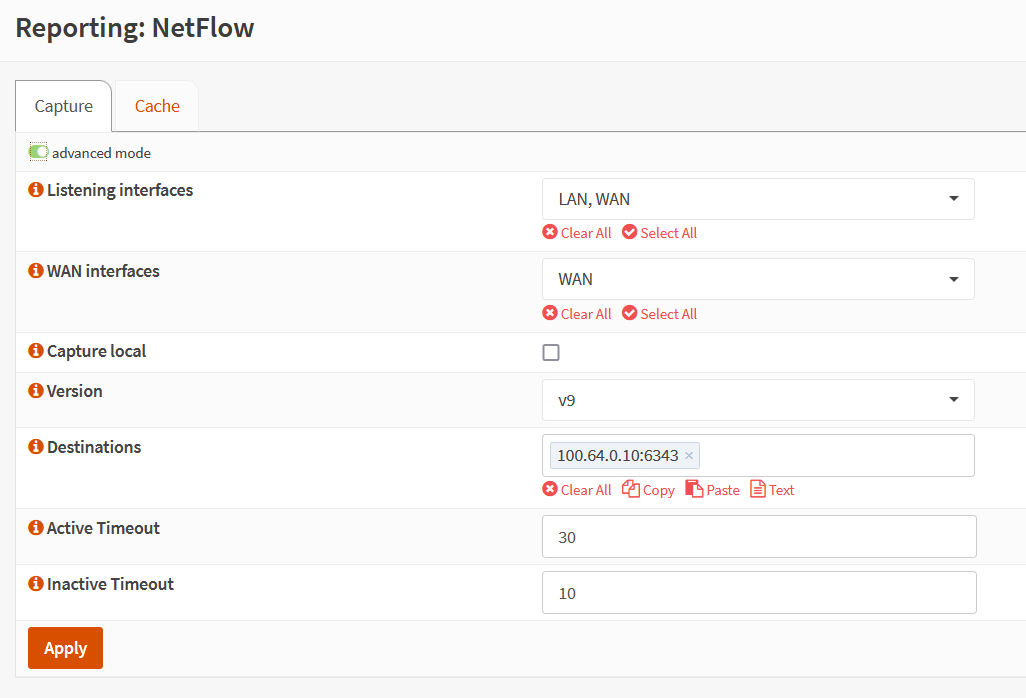
\includegraphics[width=\textwidth]{./graphics/opnsense_netflow_conf.PNG}
    \caption[OPNsense NetFlow configuratie]{elaborate description}
    \label{fig:FirewallNetflow}
\end{figure}

\paragraph{Het aanpassen van de ephemeral port range van de firewall}
De OPNsense firewall draait onderliggend FreeBSD. In onderstaande screenshot geven we aan welke port range de firewall voor zijn eigen werking mag gebruiken. De Carrier-Grade NAT moet immers deterministisch zijn. Alle combinaties ‘IP + port’ moeten bijgevolg uniek gebruikt worden. Zo mogen niet alleen tenants geen combinaties dubbel gebruiken, maar ook de firewall mag geen combinaties gebruiken die door een tenant gebruikt worden. Hiertoe geven we de firewall zijn eigen port range.

\begin{figure}[!htbp]
    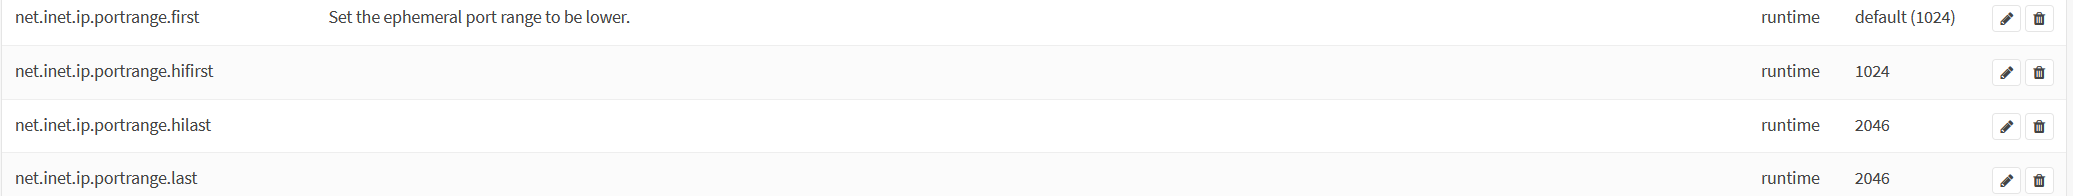
\includegraphics[width=\textwidth]{graphics/opnsense_tunables_portrange.PNG}
    \caption[OPNsense tunables portrange]{elaborate description}
    \label{fig:FirewallTunables}
\end{figure}

\paragraph{Het aanmaken van de Carrier-Grade NAT-rules op de firewall via de API}
Onderstaande screenshot geeft alle Carrier-Grade NAT rules weer die op de firewall werden geïmplementeerd. Deze rules werden opgebouwd met behulp van een Python script.

\begin{figure}[!htbp]
    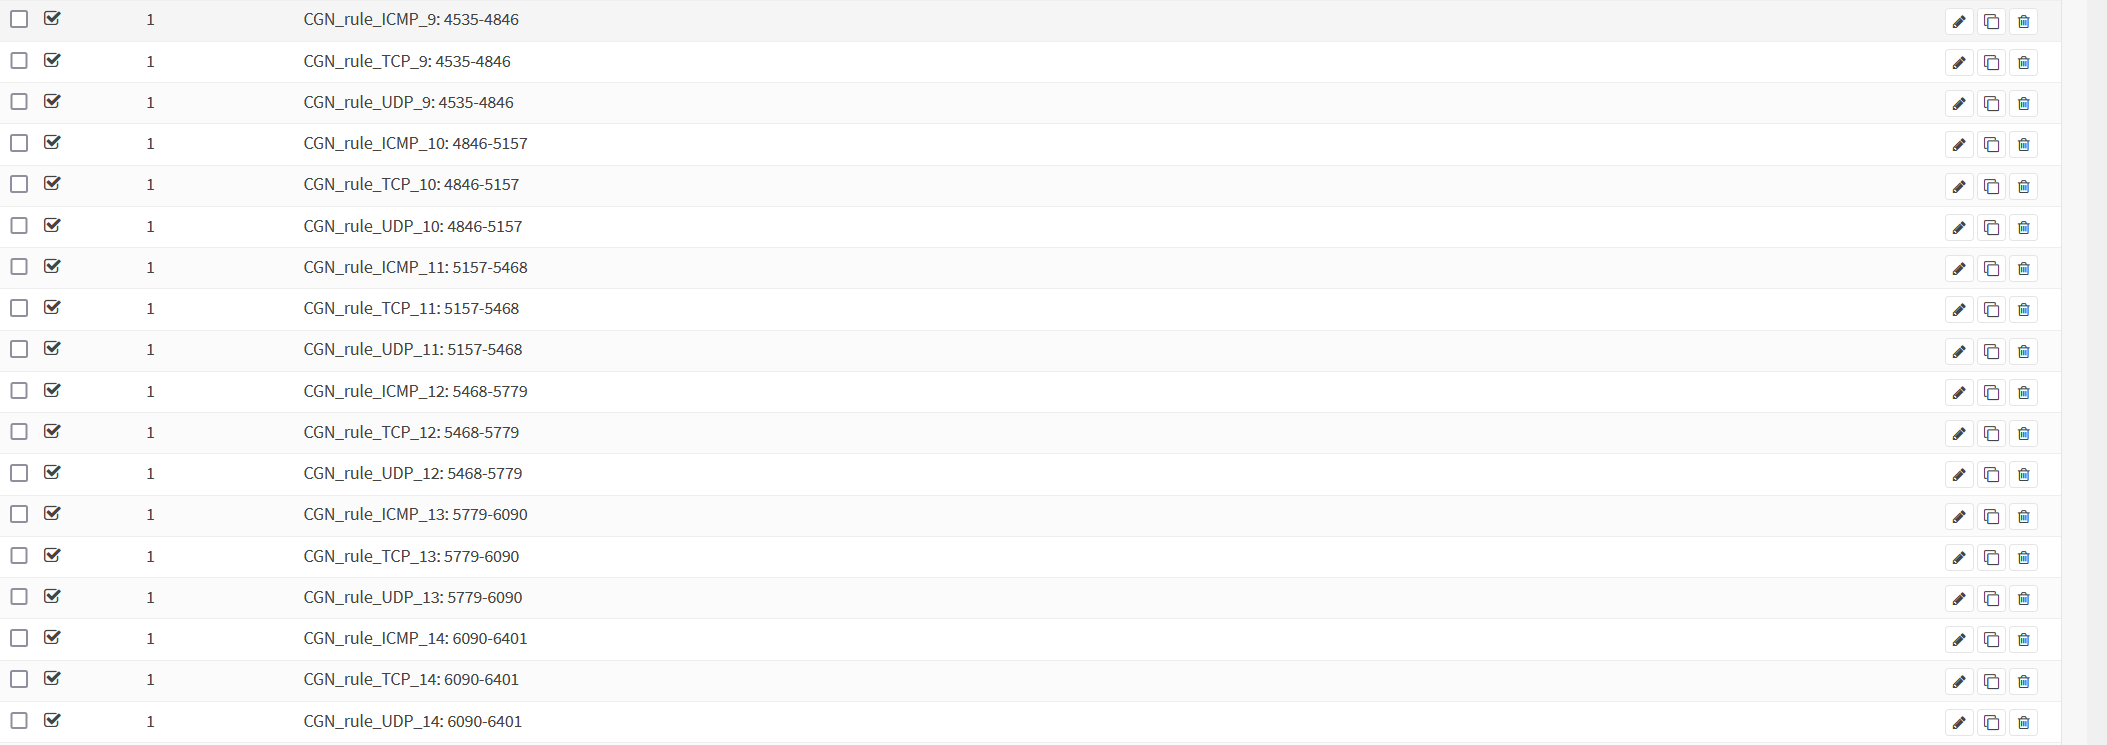
\includegraphics[width=\textwidth]{graphics/opnsense_cgnat_rules.PNG}
    \caption[OPNsense met CGN regels]{elaborate description}
    \label{fig:FirewallCGNRules}
\end{figure}

Het Python script dat hierna wordt weergegeven, genereert alle vereiste rules. In totaal zijn dit er snel enorm veel, namelijk het aantal tenants maal 3, gezien elke rule moet gelden voor zowel ICMP, UDP als TCP.

\paragraph{}
Het script bevat volgende variabelen:

\begin{itemize}
    \item Het aantal beschikbare poorten, namelijk $2^{16}$.
    \item De gereserveerde (en dus niet bruikbare) systeempoorten 0 t/m 1023.
    \item De port range die door de firewall zelf gebruikt wordt.
    \item Het aantal tenants dat dient geconnecteerd te worden.
\end{itemize}

Op basis van deze informatie berekent het script hoeveel poorten er maximaal per tenant kunnen worden toegewezen.
Vervolgens gaat het script aan elke tenant een range toekennen.
Per range worden dan drie API calls richting de firewall gelanceerd om voor zo voor elke range een ICMP, UDP en TCP source NAT rule aan te maken.

\begin{minted}{python}
    import json
    import os

    import dotenv
    import requests
    import urllib3

    urllib3.disable_warnings()

    dotenv.load_dotenv('credentials.env')
    credentials = {'key': os.environ['API_KEY'], 'secret': os.environ['API_SECRET'],
        'base_url': os.environ['API_BASE_URL']}

    total_amount_ports = (2 ** 16) - 1
    system_ports = 1023
    firewall_ports = 1023
    amount_of_CPEs = 204


    def create_url(module, controller, command, base_url=credentials['base_url'], parameters=''):
    url = f'{base_url}/{module}/{controller}/{command}/{parameters}'

    return url


    def api_call(url, request_method, verify=False, auth=(credentials['key'], credentials['secret']), json=None):
    if request_method == 'POST':
    if json:
    r = requests.post(url=url, verify=verify, auth=auth, json=json)

    else:
    r = requests.post(url=url, verify=verify, auth=auth)

    elif request_method == 'GET':
    r = requests.get(url=url, verify=verify, auth=auth)

    return r


    def get_amount_cgn_ips(ports_per_CPE, total_amount_ports=total_amount_ports, system_ports=system_ports,
    firewall_ports=firewall_ports):
    port_range_list = []

    for index, port_range in enumerate(range(system_ports + firewall_ports + 1, total_amount_ports + 1, ports_per_CPE)):
    port_range_end = port_range + ports_per_CPE

    if port_range_end < total_amount_ports:
    port_range_list.append(f'{port_range}-{port_range_end}')

    cgn_ip_count = len(port_range_list)

    return cgn_ip_count, port_range_list


    def get_amount_ports_cpe(amount_of_CPEs):
    ports_per_CPE = (total_amount_ports - (system_ports + firewall_ports)) // amount_of_CPEs
    return get_amount_cgn_ips(ports_per_CPE)


    ports = get_amount_ports_cpe(amount_of_CPEs)

    s = api_call(create_url(module='firewall', controller='filter', command='savepoint'), 'POST')
    savepoint = json.loads(s.text)['revision']
    print(f'{s.status_code}\n{s.text}')

    for index, port_range in enumerate(ports[1]):
    first_octet = 100
    second_octet = 64 + ((index + 1) // 255 ** 2)
    third_octet = (index + 1) // 255
    last_octet = (index + 1) % 255

    _, port_range_last = port_range.split("-")

    if int(port_range_last) < total_amount_ports and second_octet <= 127:
    data = {
        "rule": {
            "interface": "wan",
            "source_net": f"{first_octet}.{second_octet}.{third_octet}.{last_octet}/32",
            "target": "wanip",
            "categories": "ae1d4052-c3b4-4e21-b8f6-f7962a4b18ef"
        }
    }
    data["rule"]["protocol"] = "ICMP"
    data["rule"]["description"] = f"CGN_rule_ICMP_{index + 1}: {port_range}"
    r = api_call(create_url(module='firewall', controller='source_nat', command='addRule'), 'POST', json=data)
    print(f'{r.status_code}\n{r.text}')

    data["rule"]["protocol"] = "TCP"
    data["rule"]["description"] = f"CGN_rule_TCP_{index + 1}: {port_range}"
    data["rule"]["target_port"] = f"{port_range}"
    r = api_call(create_url(module='firewall', controller='source_nat', command='addRule'), 'POST', json=data)
    print(f'{r.status_code}\n{r.text}')

    data["rule"]["protocol"] = "UDP"
    data["rule"]["description"] = f"CGN_rule_UDP_{index + 1}: {port_range}"
    data["rule"]["target_port"] = f"{port_range}"
    r = api_call(create_url(module='firewall', controller='source_nat', command='addRule'), 'POST', json=data)
    print(f'{r.status_code}\n{r.text}')

    s = api_call(create_url(module='firewall', controller='filter', command='apply', parameters=savepoint), 'POST')
    print(f'{s.status_code}\n{s.text}')

    s = api_call(create_url(module='firewall', controller='filter', command='cancelRollback', parameters=savepoint), 'POST')
    print(f'{s.status_code}\n{s.text}')
\end{minted}
\begin{listing}[!htbp]
    \caption[Python CGN code]{elaborate description}
    \label{code:PythonCGN}
\end{listing}

\subsection{nProbe}
\begin{listing}[!htbp]
    \caption[nProbe configuration]{elaborate description}
    \label{code:nProbeConf}

    \begin{minted}{bash}
        --collector-port=6343
        --ntopng=zmq://100.64.0.11:5556
        --zmq-probe-mode
        -T="@NTOPNG@"
    \end{minted}
\end{listing}

\subsection{ntopng}
\begin{listing}[!htbp]
    \caption[ntopng configuration]{elaborate description}
    \label{code:ntopngConf}

    \begin{minted}{bash}
        --interface=tcp://*:5556c
        --https-port=3001
        --http-port=0
        --local-networks=100.64.0.0/10
    \end{minted}
\end{listing}

\section{Test}
We willen met deze test verdachte activiteit door een tenant simuleren. We doen dit door het draaien een nmap scan naar een adres dat aan de andere kant van de firewall gelegen is vanop de (arbitrair gekozen) server met IP 100.64.0.11 en port range 5157 - 5468, waar in dit geval ook ntopng op draait. Bij deze opzet werd het IP statisch toegekend.

\subsection{Carrier-Grade NAT’ing}
Onderstaande output is het resultaat een ‘sudo nmap -p- 192.168.10.1’. Op deze screenshot zien we dat de NAT’ing effectief gebeurt op de firewall.

\begin{figure}[H]
    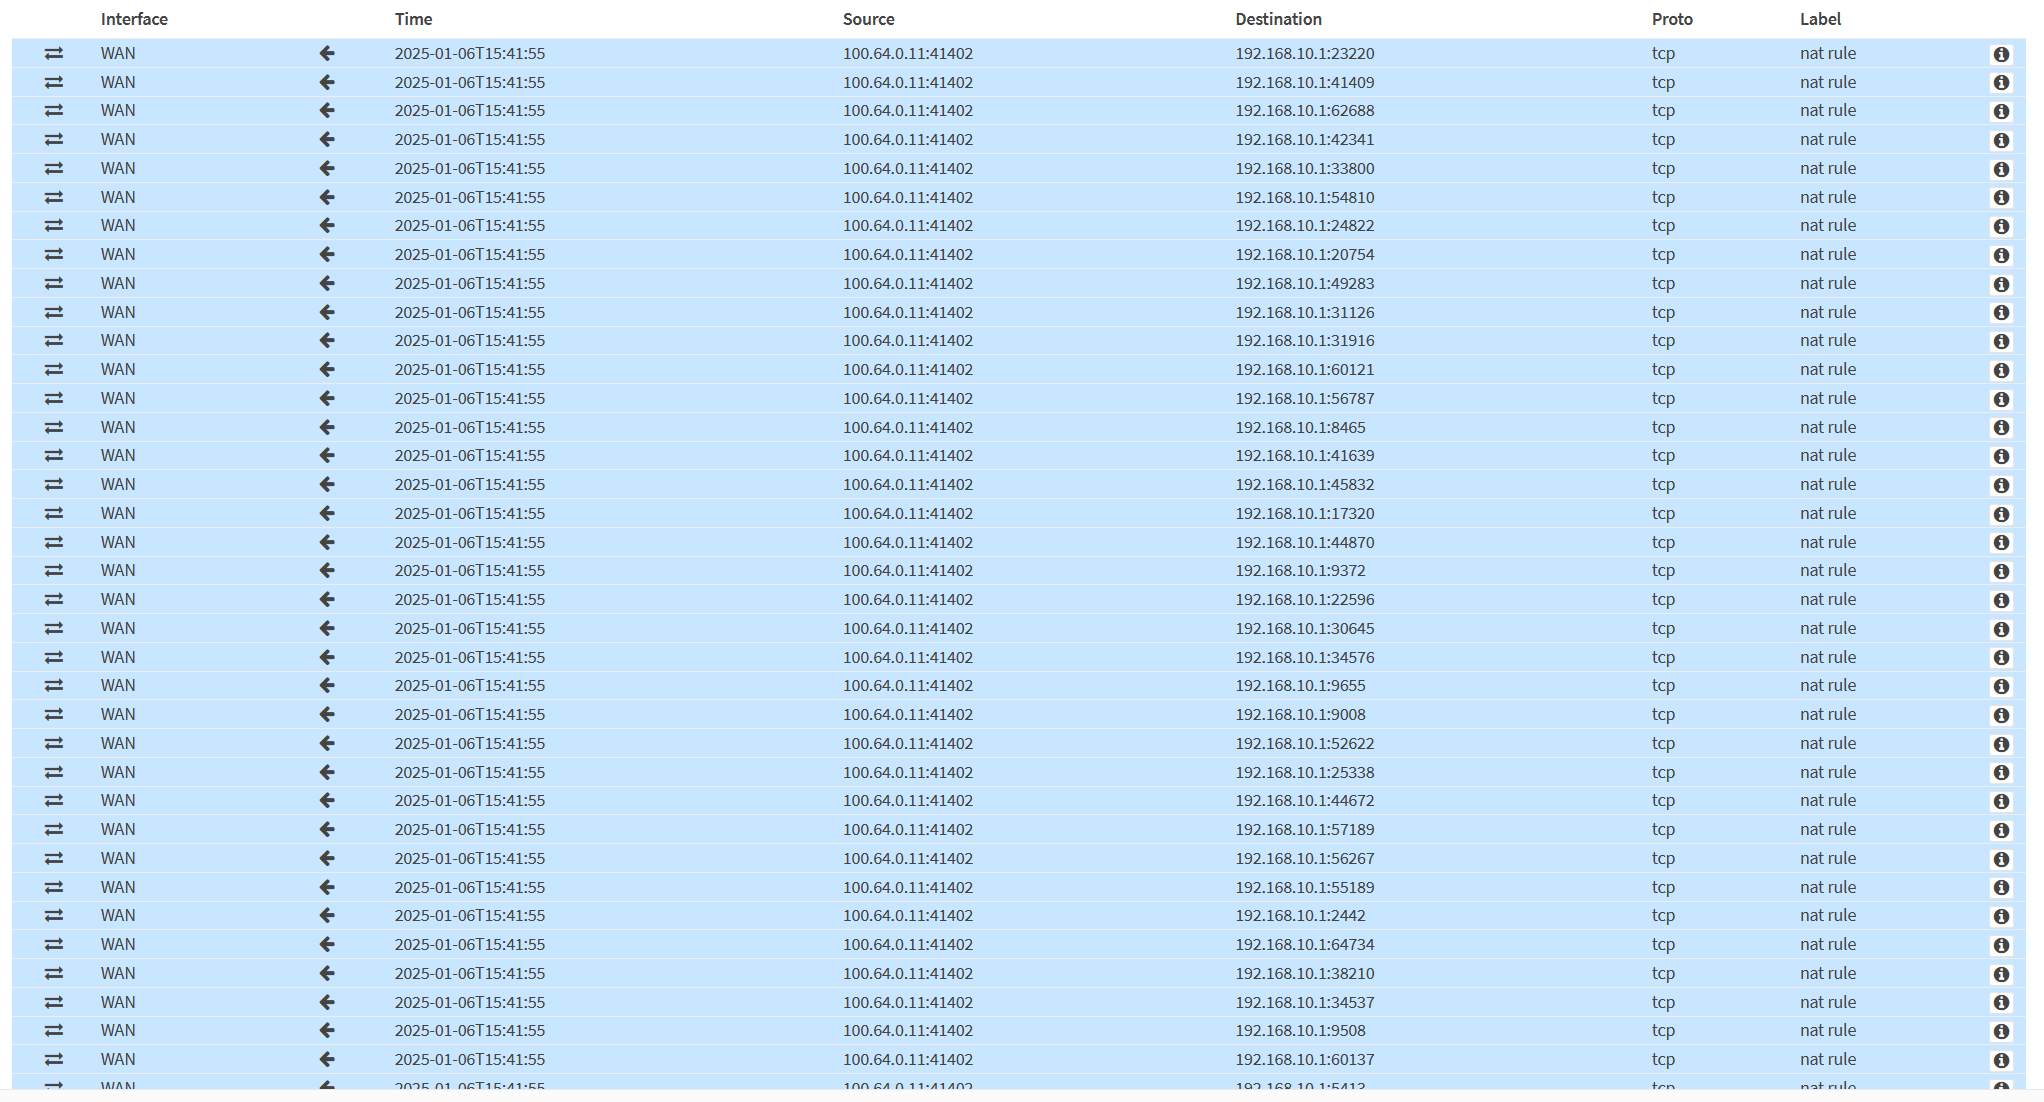
\includegraphics[width=\textwidth]{graphics/nmap_nat_table.PNG}
    \caption[OPNsense CGN regels in werking deel 1]{elaborate description}
    \label{fig:FirewallGCNWorksA}
\end{figure}

\subsection{Resultaat Carrier-Grade NAT’ing}
Onderstaande screenshot geeft de doorgelaten ge-NAT’te trafiek weer. Bemerk dat alle trafiek zich (zoals gedefinieerd en dus verwacht) binnen de source port range 5157 – 5468 bevindt.

\begin{figure}[H]
    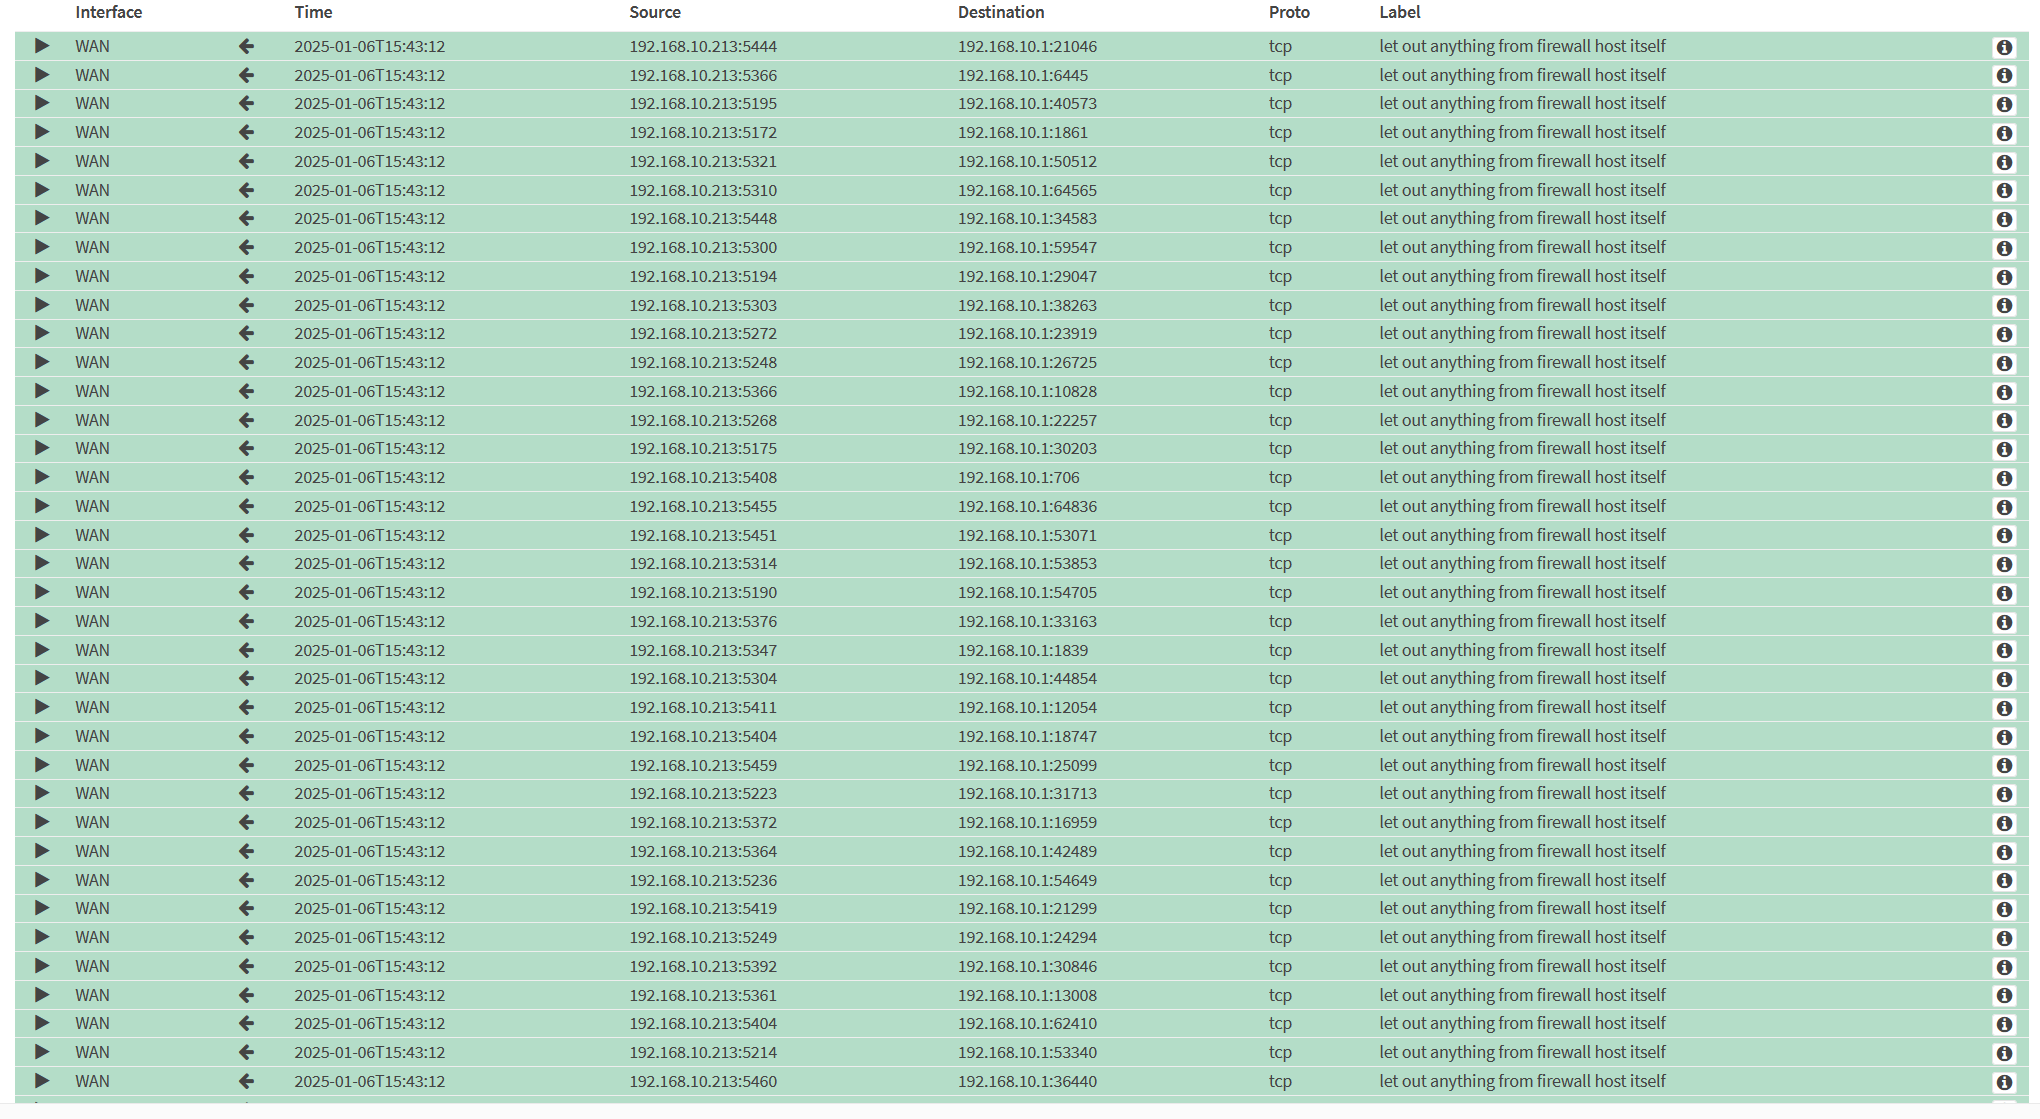
\includegraphics[width=\textwidth]{graphics/nmap_firewall_table.PNG}
    \caption[OPNsense CGN regels in werking deel 2]{elaborate description}
    \label{fig:FirewallGCNWorksB}
\end{figure}

\subsection{Geëxporteerde flows komen binnen op ntopgn}
De doorgelaten ge-NAT’te trafiek binnen de source port range 5157 – 5468 wordt door de firewall geëxporteerd naar de nProbe flowcollector die de data formatteert en vervolgens naar de ntopng flow analyser doorstuurt. Op ntopng resulteert dit in onderstaande screenshot.

\begin{figure}[htb]
    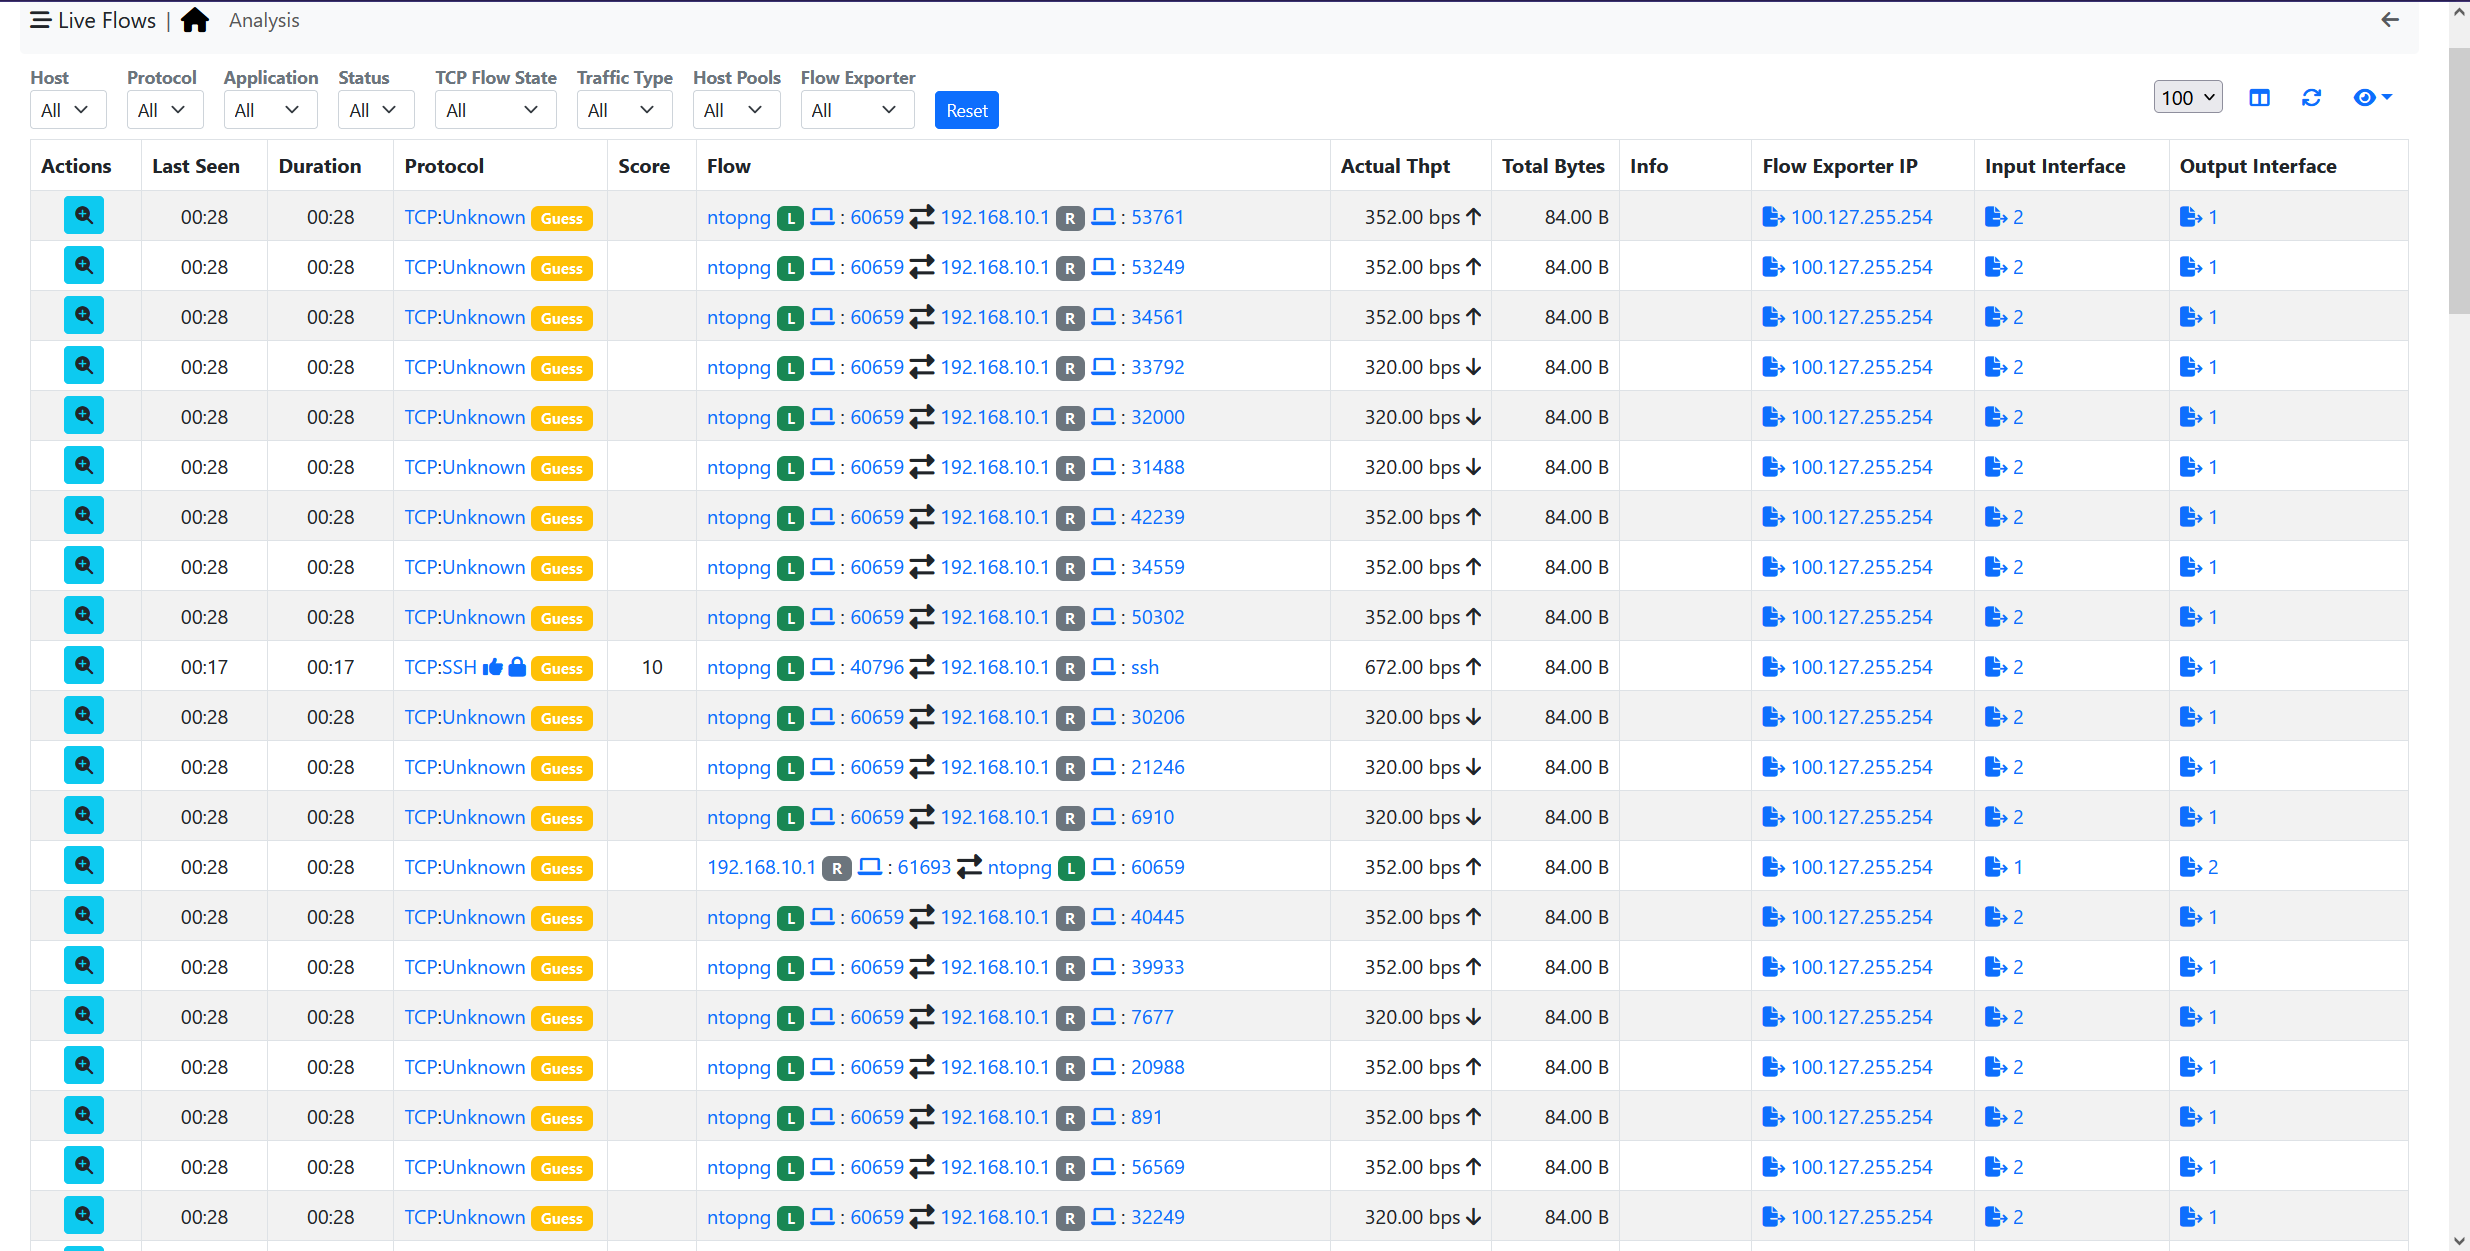
\includegraphics[width=\textwidth]{graphics/nmap_scan_flows.PNG}
    \caption[ntopng met toekomende flows]{elaborate description}
    \label{fig:ntopngFlows}
\end{figure}

\subsection{Overzicht alerts}
Tot slot is het nu ntopng die zorgt voor de beoogde behavioural checks. Hier concludeert hij met hoge severity (100) dat er vanop de server waarop ntopng draait, scanning-activiteit gaande is. In de beschrijving geeft hij bovendien aan waarom hij hiervan uitgaat: 226 scan attempts gedetecteerd, wat ruim boven het verwachtte maximum van 32 ligt.

\begin{figure}[htb]
    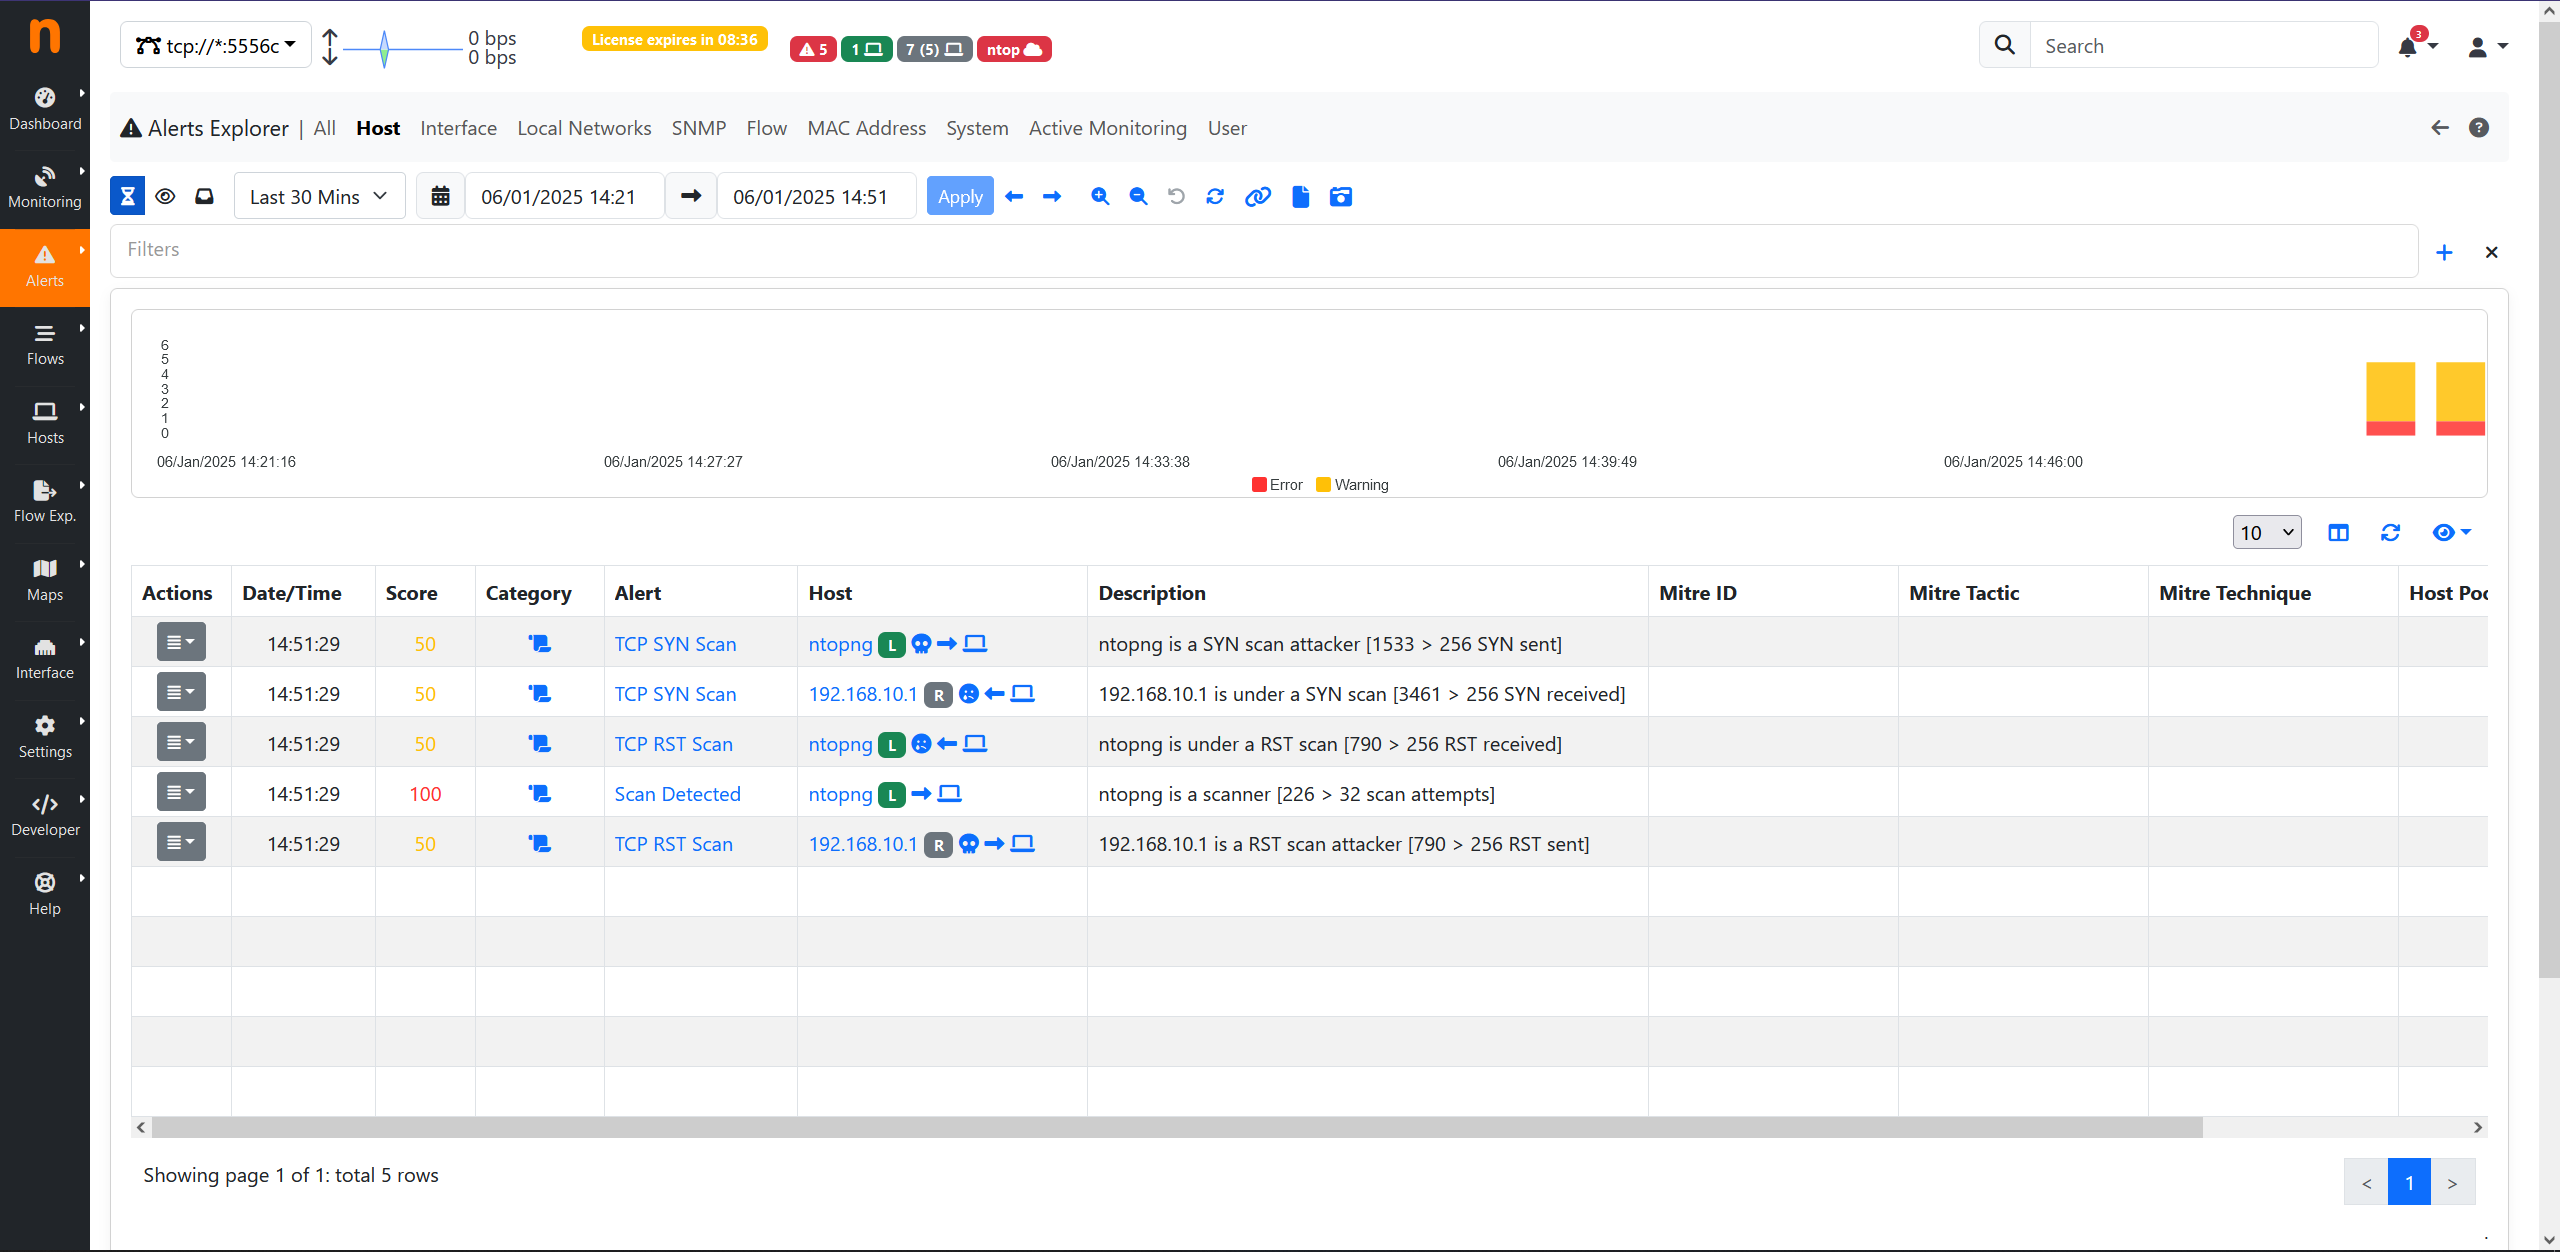
\includegraphics[width=\textwidth]{graphics/nmap_scan.PNG}
    \caption[ntopng scan alerts]{elaborate description}
    \label{fig:ntopngAlerts}
\end{figure}

%%=============================================================================
%% Conclusie
%%=============================================================================

\chapter{Conclusie}%
\label{ch:conclusie}

% TODO: Trek een duidelijke conclusie, in de vorm van een antwoord op de
% onderzoeksvra(a)g(en). Wat was jouw bijdrage aan het onderzoeksdomein en
% hoe biedt dit meerwaarde aan het vakgebied/doelgroep?
% Reflecteer kritisch over het resultaat. In Engelse teksten wordt deze sectie
% ``Discussion'' genoemd. Had je deze uitkomst verwacht? Zijn er zaken die nog
% niet duidelijk zijn?
% Heeft het onderzoek geleid tot nieuwe vragen die uitnodigen tot verder
%onderzoek?



%---------- Bijlagen -----------------------------------------------------------

\appendix

\chapter{Onderzoeksvoorstel}

Het onderwerp van deze bachelorproef is gebaseerd op een onderzoeksvoorstel dat vooraf werd beoordeeld door de promotor. Dat voorstel is opgenomen in deze bijlage.

%% TODO:
%\section*{Samenvatting}

% Kopieer en plak hier de samenvatting (abstract) van je onderzoeksvoorstel.

% Verwijzing naar het bestand met de inhoud van het onderzoeksvoorstel
%---------- Inleiding ---------------------------------------------------------

\section{Introductie}%
\label{sec:introductie}
SmartEye is een netwerk serviceprovider die Infrastructure as a Service voor projecten vanaf 8 aansluitingen aanbiedt in hetzelfde gebouw, ongeacht de mix van individuele appartementen, studentenkamers, commerciële ruimten tot gemeenschap zoals kantoren, co-working, lift, tuin, parking.~\autocite{Smarteye2021}

Als telecomoperator dient SmartEye te voldoen aan een reeks verplichtingen, opgelegd door het BIPT (Belgisch Instituut voor postdiensten en telecommunicatie). Zo is op een niet-exhaustieve lijst onder ‘Verplichtingen rond (persoons)\-gegevens en privacy / Identificatie van eindgebruikers’ volgende verplichting terug te vinden: “Een operator is verplicht de abonnees op zijn elektronische communicatiediensten te identificeren (directe identificatiemethode), of er ten minste voor te zorgen dat de autoriteiten hen kunnen identificeren (indirecte identificatiemethode).”~\autocite{BIPT2023}

Stel nu dat bevoegde overheidsinstanties een threat kunnen backtracen tot een door SmartEye beheerde netwerkomgeving, kan SmartEye vervolgens de locatie (een ruimte binnen het gebouw) van de potentële threat actor identificeren?

Aansluitend bij deze vraag wil SmartEye logischerwijze ook proactief kunnen inspelen op potentiële vragen van de bevoegde overheidsinstanties door mogelijke threats ten allen tijde reeds zelf te onderkennen.

Aan de hand van een literatuurstudie en een proof of concept (PoC) willen we een antwoord geven op bovenstaande onderzoeksvraag. Met betrekking tot de bijkomende vraag van Smart\-Eye, zal de PoC zich echter wel beperken tot het detecteren van netwerkscans als threats, om vervolgens de threat actors te identificeren binnen de door SmartEye beheerde netwerken.
%---------- Stand van zaken ---------------------------------------------------

\section{Stand van zaken}%
\label{sec:state-of-the-art}

\subsection{Netwerkoverwegingen}

\paragraph{Publieke IPv4 adressen}
\emph{Kan SmartEye niet iedereen gewoon een publiek IPv4 geven? }

Neen. Zo goed als alle beschikbare IPv4-ranges werden immers reeds door het IANA~\autocite{ICANN2012} en de onderliggende Regional Internet Registries\\\autocite{Gerich1993} (RIR’s) uitgedeeld. Voor België gebeurde dit door het RIPE NCC.

Op 25 november 2019 echter, kondigde het \textcite{RIPE_NCC2019}  aan dat alle beschikbare ranges (/8, /22 of /22 als combinatie van /23’s en/of /24’s) uitgeput waren. Local Internet Registries (LIR’s) kunnen zich enkel nog voor een wachtlijst aanmelden om eventueel ooit één /24 te bekomen.

Getuige van dit schrijnend tekort is het statement van~\textcite{Neuckens2022} bij Proximus, dat zij hun laatste IPv4-blok van het RIPE NCC ontvingen in 2012.

\paragraph{NAT}
\emph{Hoe kunnen we dit oplossen binnen een IPv4-context?}

Traditionele Network Address Translation (NAT) stelt hosts binnen een privé-netwerk~\autocite{Moskowitz1996} in staat om transparant toegang te krijgen tot hosts in het externe netwerk (zoals het internet).

NAPT~\autocite{Holdrege1999} breidt het begrip ‘translation’ een stap verder uit door ook de transport identifier te vertalen (bijv. TCP en UDP poortnummers en ICMP query identifiers). Hierdoor kunnen de transport identifiers van een aantal privé-hosts gemultiplext worden tot de\\transport identifiers van een enkel extern adres. Met NAPT kan een verzameling hosts dus een enkel extern adres delen.

\paragraph{Carrier-Grade NAT}
SmartEye krijgt door een Internet Service Provider (ISP) per locatie één binnenkomend publiek IP, dat gedeeld wordt door meerdere tenants (huurders, eindgebruikers).\\ Daarom dienen alle NAT-translaties deterministisch~\autocite{Donley2014} te zijn ofwel gelogd~\autocite{Perreault2013} te worden indien deze dynamisch zijn. Zodoende wordt Carrier-Grade NAT geïmplementeerd. Identificatie van de potentiële threat actor is anders immers niet mogelijk.

\paragraph{Publieke IPv6 adressen}
\emph{Kunnen we dit oplossen door over te stappen op IPv6-context?}

Ja. Echter, vanuit een IPv6-context moet men nog steeds het IPv4 gebaseerde deel van het internet kunnen bereiken. Hoewel hiervoor door de Internet Engineering Task Force (IETF) oplossingen~\autocite{Arkko2011} werden uitgewerkt, blijft de vereiste geldig dat een en ander deterministisch dient te gebeuren of gelogd moet worden. Bovendien is het essentieel om aan te stippen dat SmartEye vandaag de dag IPv4 only is.

\subsection{Datacaptatie en -export}
\emph{Welke technologieën kunnen nu het loggen van NAT-translaties faciliteren en een zicht geven op verdachte netwerktrafiek?}

\paragraph{Netflow}
NetFlow werd door Cisco ontwikkeld als feature voor zijn routers. Essentiële versies zijn versie 5, die IPv4 only is, en versie 9, die zowel met IPv4 als IPv6 overweg kan. Waar bij versie 5~\autocite{Cisco2007} de velden qua inhoud vastliggen, is versie 9~\autocite{Claise2004} template gebaseerd waardoor de inhoud van de velden toewijsbaar is.
\paragraph{IPFIX}
IPFIX (Internet Protocol Flow Information Export)~\autocite{Aitken2013} is dan weer een door het IETF uitgewerkte standaard, gebaseerd op Netflow versie 9. De specificaties zijn terug te vinden in de RFC’s 7011 tot en met RFC 7015, en in RFC 5103.
\paragraph{sFlow}
Waar bij NetFlow en IPFIX een pakket-\\aggregatie op layer 3 plaatsgrijpt, vindt er bij sFlow sampling plaats op layer 2. sFlow~\autocite{Phaal2004} werd ontwikkeld door InMon Corporation.

% Voor literatuurverwijzingen zijn er twee belangrijke commando's:
% \autocite{KEY} => (Auteur, jaartal) Gebruik dit als de naam van de auteur
%   geen onderdeel is van de zin.
% \textcite{KEY} => Auteur (jaartal)  Gebruik dit als de auteursnaam wel een
%   functie heeft in de zin (bv. ``Uit onderzoek door Doll & Hill (1954) bleek
%   ...'')S

%---------- Methodologie ------------------------------------------------------
\section{Methodologie}%
\label{sec:methodologie}

We opteren voor een \textbf{proof of concept} (PoC) die zich zal beperken tot het detecteren van netwerkscans als threats, om vervolgens de threat actors te identificeren binnen de door SmartEye beheerde netwerken. Niet de volledigheid van de oplossing, maar de correctheid en werkbaarheid moet immers aangetoond worden.

Vanuit ook de businessvereiste om tot een oplossing te komen met een minimale kost, zal er voor geopteerd worden om de oplossing op basis van deterministische NAT-translaties in eerste instantie verder uit te werken. Aan het loggen van alle translaties hangt immers een stevig storageprijskaartje. Het BIPT vereist immers om over de historiek van een jaar te beschikken.

Op basis van een \textbf{literatuurstudie} zal eerst de haalbaarheid van een op deterministische NAT-translaties gebaseerde oplossing bekeken worden. Vervolgens zal de haalbaarheid effectief getest worden aan de hand van een PoC. Ook zal de literatuurstudie de mogelijkheden van IPv4 versus IPv6 onderzoeken.

\subsection{MoSCoW-analyse}

Een eerste MoSCoW-analyse brengt reeds volgende inzichten op functioneel vlak:
\begin{itemize}
    \item Must have
        \begin{itemize}
            \item Detecteren van threats
            \item Identificeren van threat actors
        \end{itemize}
    \item Should have
        \begin{itemize}
            \item DHCP-logging omdat louter de NAT-\\informatie onvoldoende is voor identificatie binnen een DHCP-gebaseerd netwerk.
        \end{itemize}
    \item Could have
        \begin{itemize}
            \item Deze werden in dit stadium van de opdracht nog niet gedetecteerd.
        \end{itemize}
    \item Won't have
        \begin{itemize}
            \item  Complexe threatdetecties. Enkel het onderkennen van netwerkscans maakt deel uit van deze PoC.
            \item Geolocatiebepalingen
        \end{itemize}
\end{itemize}

\subsection{Fasering}

\begin{itemize}
    \item Literatuurstudie
        \begin{itemize}
            \item Tijdbesteding: 50\%
            \item Deliverables: een duidelijk zicht geven op de mogelijke oplossingsrichtingen
        \end{itemize}
    \item Requirements-analyse
        \begin{itemize}
            \item Tijdbesteding: 10\%
            \item Deliverables: duidelijk aangeven wat  de preferente oplossing is
        \end{itemize}
    \item PoC
        \begin{itemize}
            \item Tijdbesteding: 40\%
            \item Deliverables: bewijs leveren van het feit dat de preferente oplossing implementeerbaar is en voldoet aan de gestelde requirements
        \end{itemize}
\end{itemize}

%---------- Verwachte resultaten ----------------------------------------------
\section{Verwacht resultaat}%
\label{sec:verwachte_resultaten}

Wanneer bevoegde overheidsinstanties een threat backtracen tot een door SmartEye beheerde netwerkomgeving, moet SmartEye vervolgens de locatie (een ruimte binnen het gebouw) van de potentële threat actor kunnen identificeren. Deze bachelorproef voorziet in deze wettelijke vereiste door een bewezen correcte en werkbare oplossing (PoC) aan te reiken die voldoet aan de vereisten die, én door de regulator gesteld worden, én door SmartEye. De meerwaarde van deze bachelorproef is bijgevolg aangetoond.

Deze bachelorproef zal mij veel bijkomend en diepgaand inzicht geven in het netwerkdomein. Het is immers duidelijk dat meerdere RFC’s, toch wel dé referentiedocumenten binnen het netwerkdomein, grondig zullen moeten doorgenomen en bestudeerd worden om tot een gefundeerde stellingname en keuze te komen.



%%---------- Andere bijlagen --------------------------------------------------
% TODO: Voeg hier eventuele andere bijlagen toe. Bv. als je deze BP voor de
% tweede keer indient, een overzicht van de verbeteringen t.o.v. het origineel.
%\input{...}

%%---------- Backmatter, referentielijst ---------------------------------------

\backmatter{}

\setlength\bibitemsep{2pt} %% Add Some space between the bibliograpy entries
\printbibliography[heading=bibintoc]

\end{document}
